\documentclass{article}

\usepackage{graphicx}
\usepackage{geometry}

\geometry{top=0.1in, left=0.1in, right=0.1in, bottom=0.1in}

\usepackage{array}
\usepackage{makecell}
\usepackage{tabularx}
\renewcommand{\tabularxcolumn}[1]{m{#1}}

\pdfpageheight=5in
\pdfpagewidth=7.2in

\begin{document}
	\begin{tabularx}{7in}{|m{1em}|X|X|X|X|}
		\hline
		& \multicolumn{1}{c|}{Visual Cue} & \multicolumn{1}{c|}{Tongue} & \multicolumn{1}{c|}{Right Foot} & \multicolumn{1}{c|}{Right Hand} \\ \hline
		\rotatebox{90}{\textbf{Bayesian GLM}}& 
		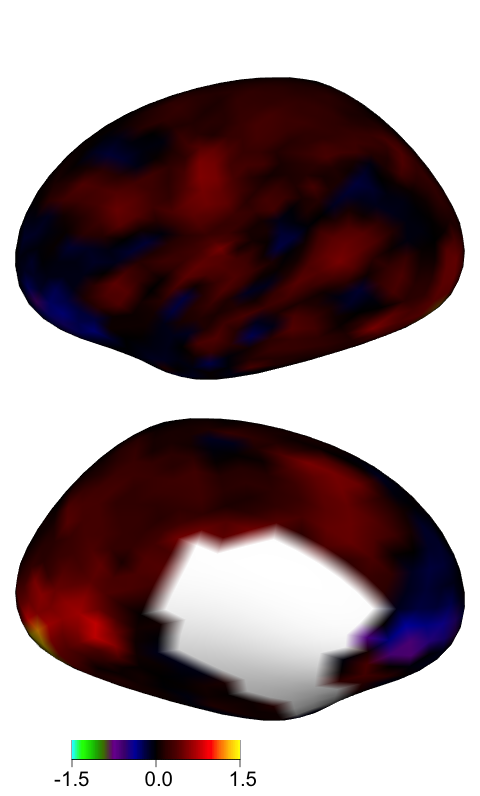
\includegraphics[width=1.5in]{plots/601_single_subject_Bayes_visual_cue.png} &
		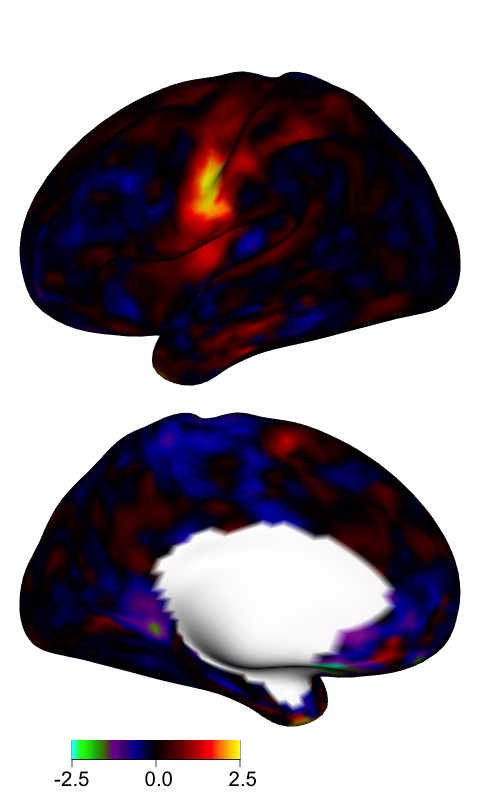
\includegraphics[width=1.5in]{plots/601_single_subject_Bayes_tongue.png} &
		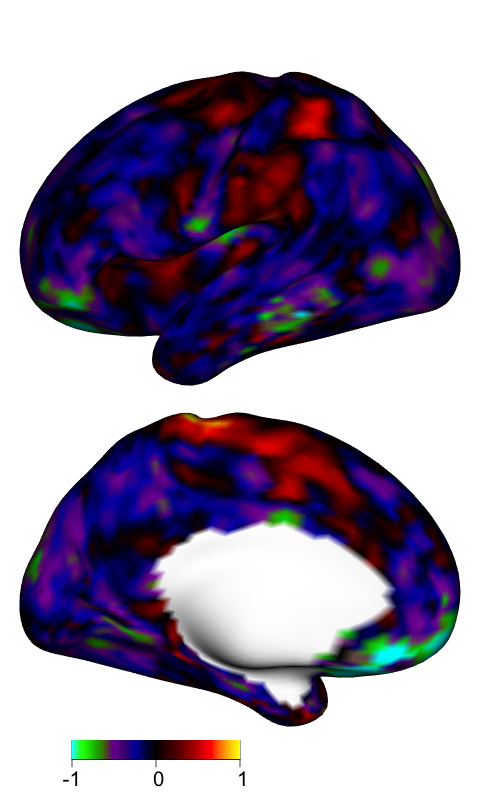
\includegraphics[width=1.5in]{plots/601_single_subject_Bayes_right_foot.png} &
		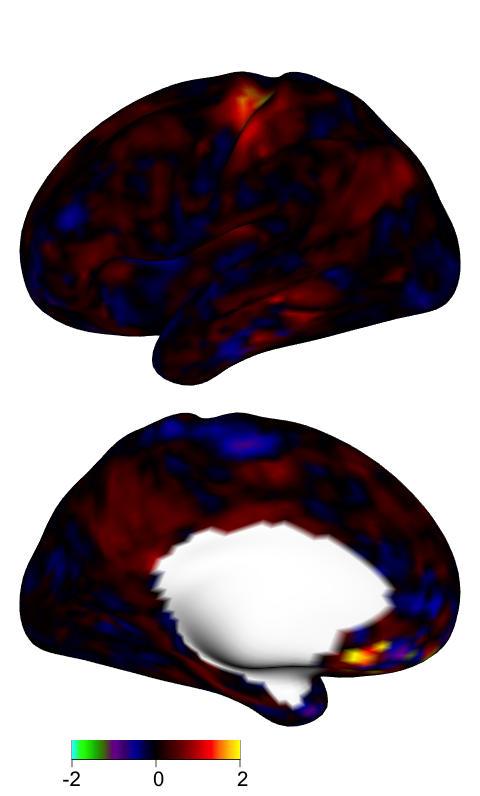
\includegraphics[width=1.5in]{plots/601_single_subject_Bayes_right_hand.png} \\ \hline
		\rotatebox{90}{\textbf{Classical GLM}} & 
		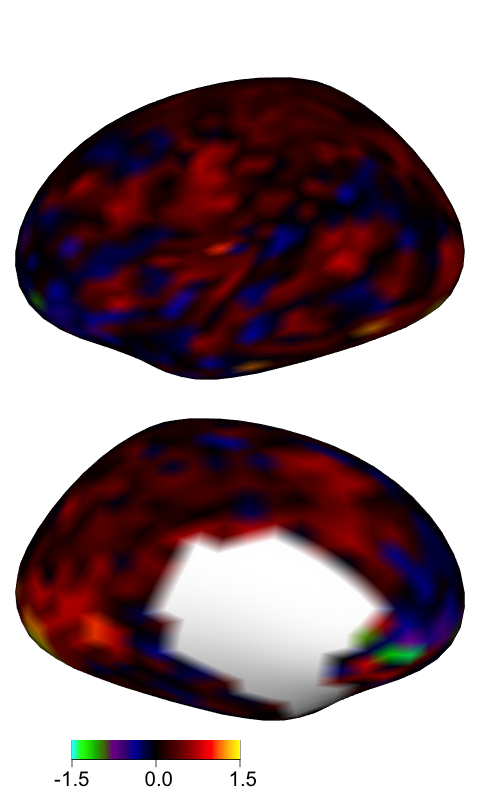
\includegraphics[width=1.5in]{plots/601_single_subject_classical_visual_cue.png} &
		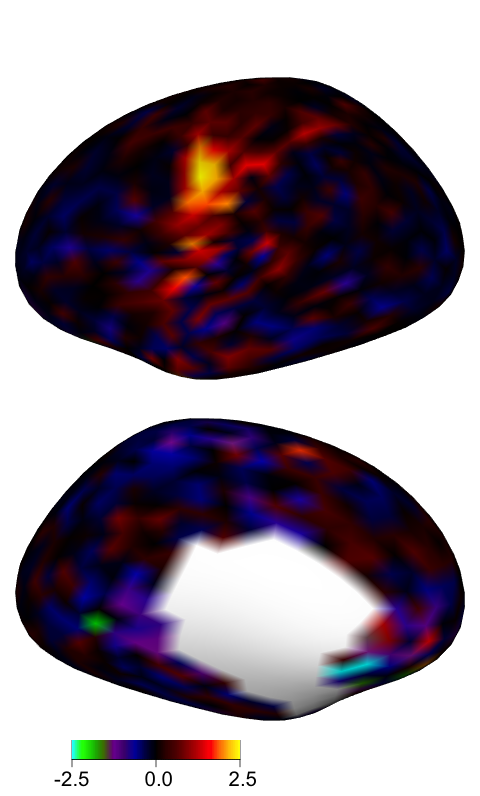
\includegraphics[width=1.5in]{plots/601_single_subject_classical_tongue.png} &
		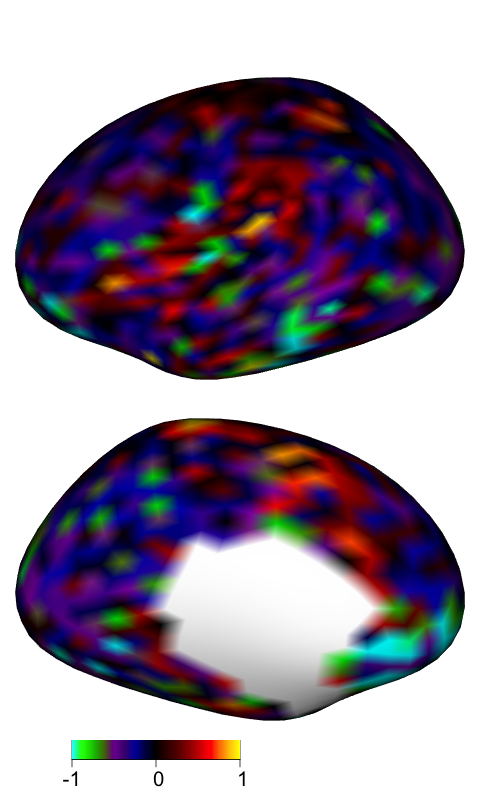
\includegraphics[width=1.5in]{plots/601_single_subject_classical_right_foot.png} &
		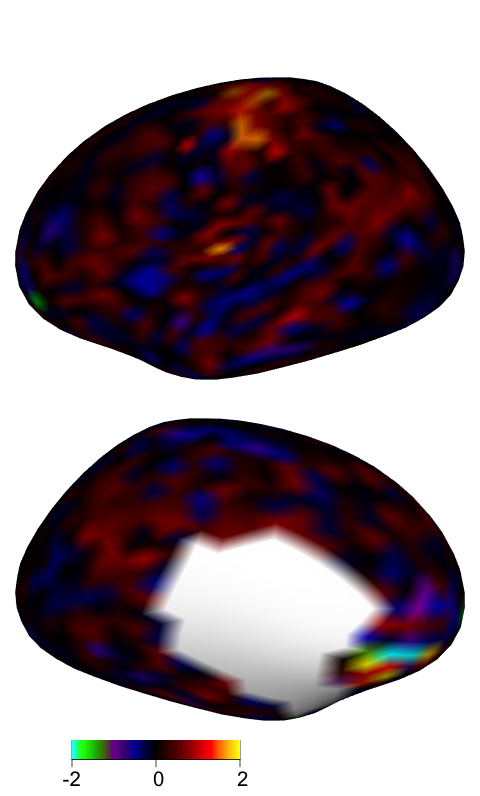
\includegraphics[width=1.5in]{plots/601_single_subject_classical_right_hand.png} \\ \hline
	\end{tabularx}
\end{document}